\chapter{Постановка задачи} \label{chapt2}

Почти все задачи машинного обучения содержат в себе три важные подзадачи:
\begin{enumerate}
    \item Сбор данных
    \item Обучение нейронной сети
    \item Решение инфраструктурных задач
\end{enumerate}

В данном проекте задача решалась итеративно, и цикл повторяется пока задача не будет считаться решённой. Причина этому - более экономная трата ресурсов и постоянная обратная связь. Если несколько циклов подряд задачу решить не получается - меняют вводные, либо меняют задачу. 

\section{Содержательная} \label{sect2_1}
\textbf{Дано: } 

Изображение или видеопоток, на котором гарантированно присутствует собака.

\textbf{Требуется: } 

Вернуть информацию о позиции собаки в данный на изображении среди следующих классов: [Стоит, сидит, лежит].

Требования к изображению и видеопотоку, которые идут на вход указанной системе. 

Собака в кадре должна быть:
\begin{itemize}
    \item Видна целиком
    \item Ничем не загорожена, даже частично
    \item На кадре находится одна
    \item Занимает более 50\% кадра по высоте или по ширине
    \item Хвост может быть загорожен телом 
    \item От собаки до края кадра есть ещё место, больше 1\% высоты и ширины кадра
 \end{itemize}
 
Камера относительно собаки:
\begin{itemize}
    \item Находится на расстоянии более 2м
    \item Смотрит на собаку на уровне глаз либо выше, но не сверху.
\end{itemize}

\section{Математическая} \label{sect2_2}
Данная задача сведена к задаче классификации изображений по N классам. Наличие собаки гарантируется на кадре. Чтобы классифицировать изображение, используется свёрточная нейронная сеть архитектуры ResNet-34 \cite{resnet}.

\begin{figure}[ht] 
  \center
  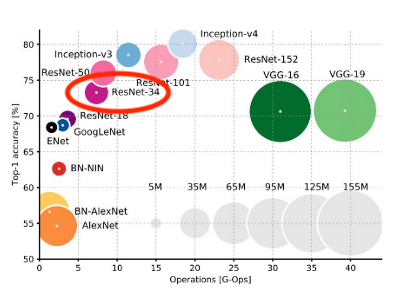
\includegraphics [scale=1] {resnet}
  \caption{Соотношение точности к сложности вычислений у ResNet-34 относительно других архитектур} 
  \label{img:resnet}  
\end{figure}
